\section{VLBI}
Very Long Baseline Interferometry - Interferometria Długich Baz jest techniką geodezji kosmicznej która powstała w latach 80 ubiegłego wieku.
Polega na obserwacji fali elektromagnetycznej w paśmie częstotliwości radiowych, która jest emitowana przez obiekty pozagalaktyczne (kwazary).\\
\indent Radio-interferometr złorzony z pary anten kierunkowych - radioteleskopów, jak na rysunku \ref{fig:vlbi_antenna}, obserwuje w zadanym przedziale czasu
tylko jedno źródło pozagalaktyczne. W typowej 24 godzinnej sesji obserwacyjnej VLBI uczestniczy zwykle 8 stacji, które obserwują 60 kwazarów kilkukrotnie w ciągu doby.
\cite[][strona 27]{ggos}.
\begin{figure}[H]
\centering
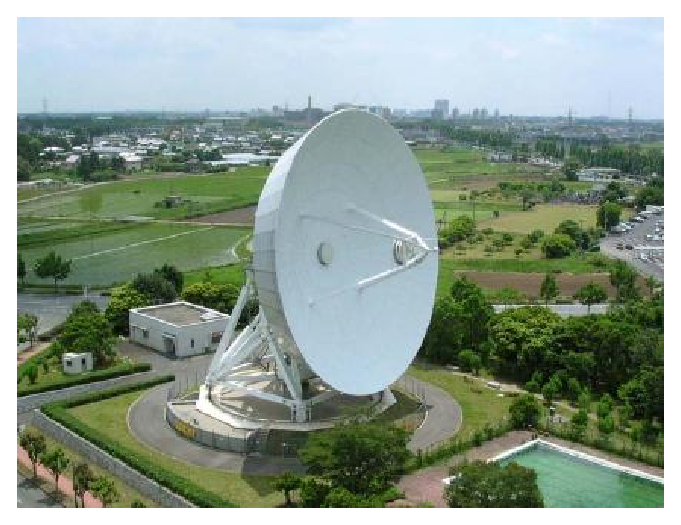
\includegraphics[scale=0.6]{appendix_vlbi_antenna.eps}
\caption{\textit{Antena VLBI o średnicy 32 metrów w mieście Tsukuba, Japonia.} źródło: \cite[][strona 28]{ggos}}
\label{fig:vlbi_antenna}
\end{figure}

\indent Kwazary są tak bardzo oddalone od Układu Słonecznego, że ich ruchy własne są niewykrywalne żadną istniejacą aparaturą. Z punktu widzenia dokładności pomiaru 
uznajemy je zatem za punkty stałe w przestrzeni kosmicznej. Zbiór pozagalaktycznych radio-źródeł realizuje zatem inercjalny układ odniesienia w oparciu o który precyzyjnie
(dokładność rzędu kilku milimetrów) estymowane są pozycje stacji VLBI. Względne prędkości stacji wyznacza się na podstawie kilkuletnich szeregów czasowych obserwacji VLBI 
\cite[][strona 27]{ggos}. Poniżej opisano procedurę wyznaczania współrzędnych wektora o początku i końcu umieszczonych w centrach fazowych radio-interferometru 
\ref{fig:vlbi_principle}.\\
\indent Sygnał radiowy odbierany przez radioteleskop stacji VLBI jest nagrywany cyfrowo z bardzo dokładną referencją czasową dostarczaną przez maser wodorowy. 
\footnote{Maser to urządzenie o zasadzie działania identycznej jak laser, ale emitujące promieniowanie w innym zakresie częstotliwości, która chartakteryzuje się 
wysoką stabilnością. 1s spóźnienia na ponad 10mln lat}
Ten sam sygnał przebywa dodatkową drogę $c\tau$ zanim dotrze do centrum fazowego drugiej anteny interferometru. Gdzie $c$ to prędkość światła, a $\tau$ stanowi 
różnicę czasu dotarcia fali radiowej do obu anten interferometru, wyznaczaną za pomocą korelacji nagranych sygnałów. W ten sposób obliczany jest rzut wektora stanowiącego bazę
na oś w kierunku do badanego radioźródła \cite[][strona 27]{ggos}. 
Na podstawie pomiarów sygnałów pochodzących od różnych radioźródeł, wyznacza się wszystkie współrzędne wektora zdefiniowanego między centrami fazowymi anten 
radiointerferometru w układzie ICRF. 
\begin{figure}[H]
\centering
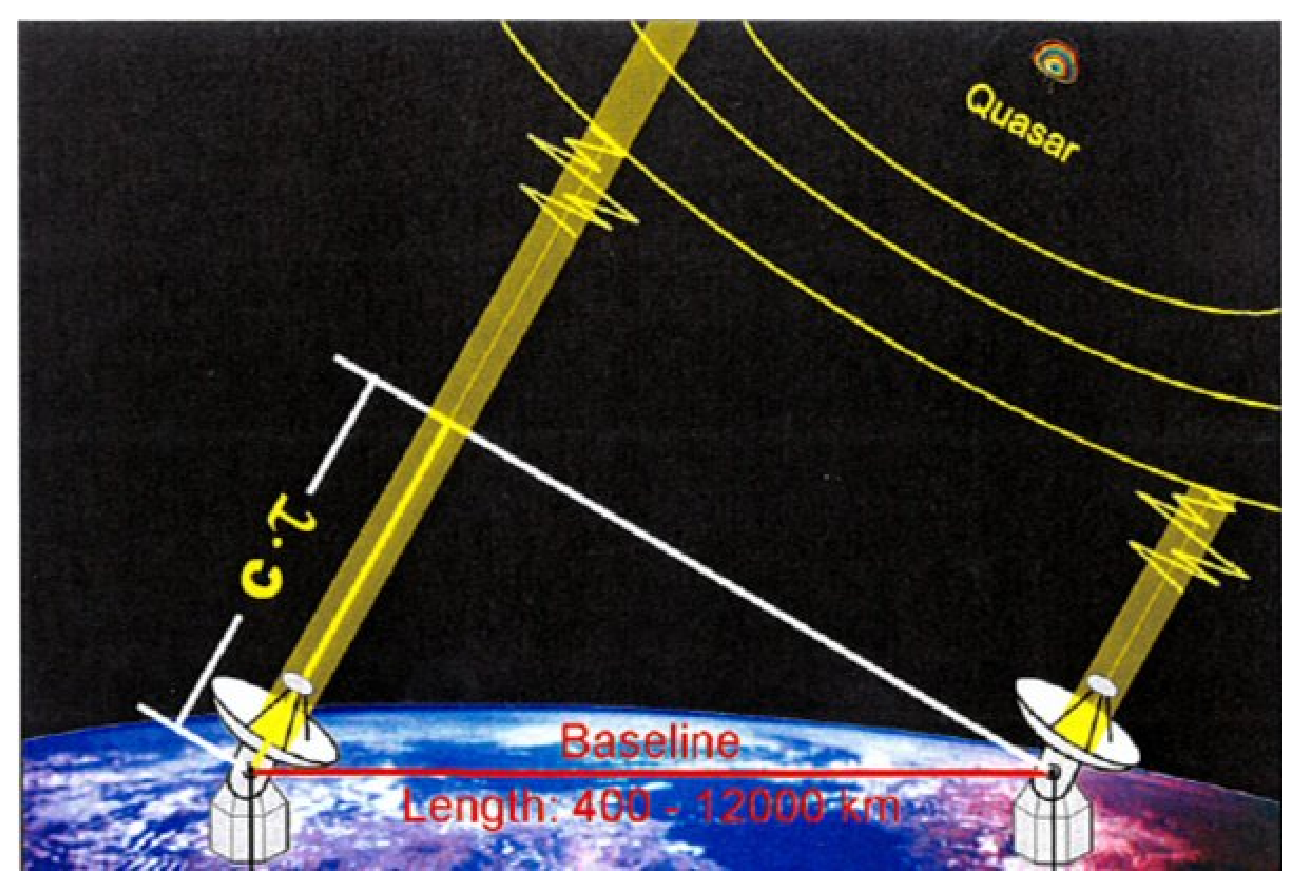
\includegraphics[scale=0.6]{appendix_vlbi_principle.eps}
\caption{\textit{Zasada działania Interferometrii Długich Baz} źródło: \protect\url{http://www.mpifr-bonn.mpg.de/technologie/vlbi}}
\label{fig:vlbi_principle}
\end{figure}



%%%%%%%%%%%%%%%%%%%%%%%%%%%%%%%%%%%%%%%%%%%%%%%%%%%%%%%%%%%%%%%%%%%%%%%%%%%%%%%%%%%%%%%%%%
%			DORIS
%%%%%%%%%%%%%%%%%%%%%%%%%%%%%%%%%%%%%%%%%%%%%%%%%%%%%%%%%%%%%%%%%%%%%%%%%%%%%%%%%%%%%%%%%%
\section{DORIS}
\noindent DORIS (Doppler Orbitography and Radiopositioning Integrated by Satellite) jest francuskim cywilnym systemem montowanym 
na satelitach, służącym głównie do precyzyjnego wyznaczania orbit sztucznych satelitów Ziemi oraz pozycjonowania aktywnych stacji referencyjnych.
Zaprojektowany przez Francuską Agencję Kosmiczną CNES, system bazuje na efekcie Dopplera zmiany częstotliwości fali radiowej rejestrowanej przez odbiornik 
umieszczony na satelicie będącym w ruchu orbitalnym, uzględem częstotliwości referencyjnej sygnału wysłanego ze stacji naziemnej sztywno związanej z Ziemią
 w jej ruchu obrotowym. \cite[]{DORIS_AVISO} System składa się z anteny długości 42 cm, radio-odbiornika oraz wysoko stabilnego generatora częstotliwości wzorcowej. 
Elementy te przedstawia rysunek \ref{fig:DORIS_equipment}.
\begin{figure}[H]
\centering
\begin{subfigure}{.33\textwidth}
  \centering
  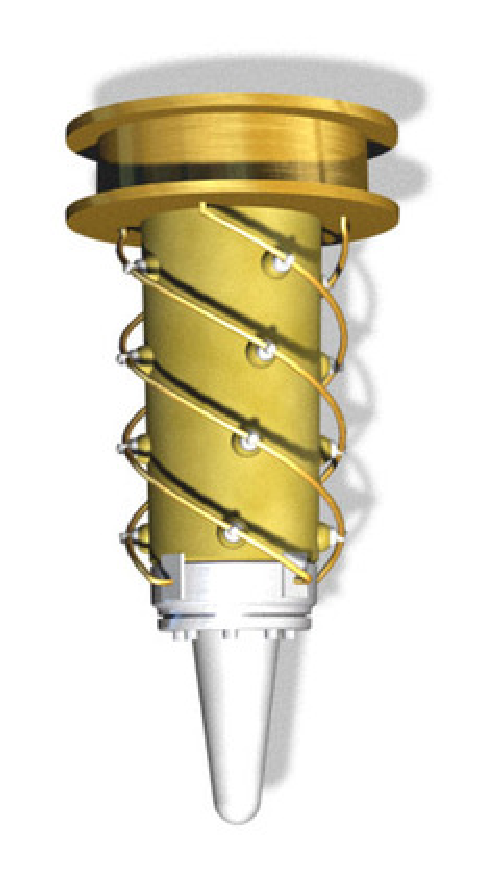
\includegraphics[width=.3\linewidth]{appendix_doris_antenna.eps}
  \caption{antena}
  \label{fig:DORIS_eq_sub1}
\end{subfigure}%
\begin{subfigure}{.3\textwidth}
  \centering
  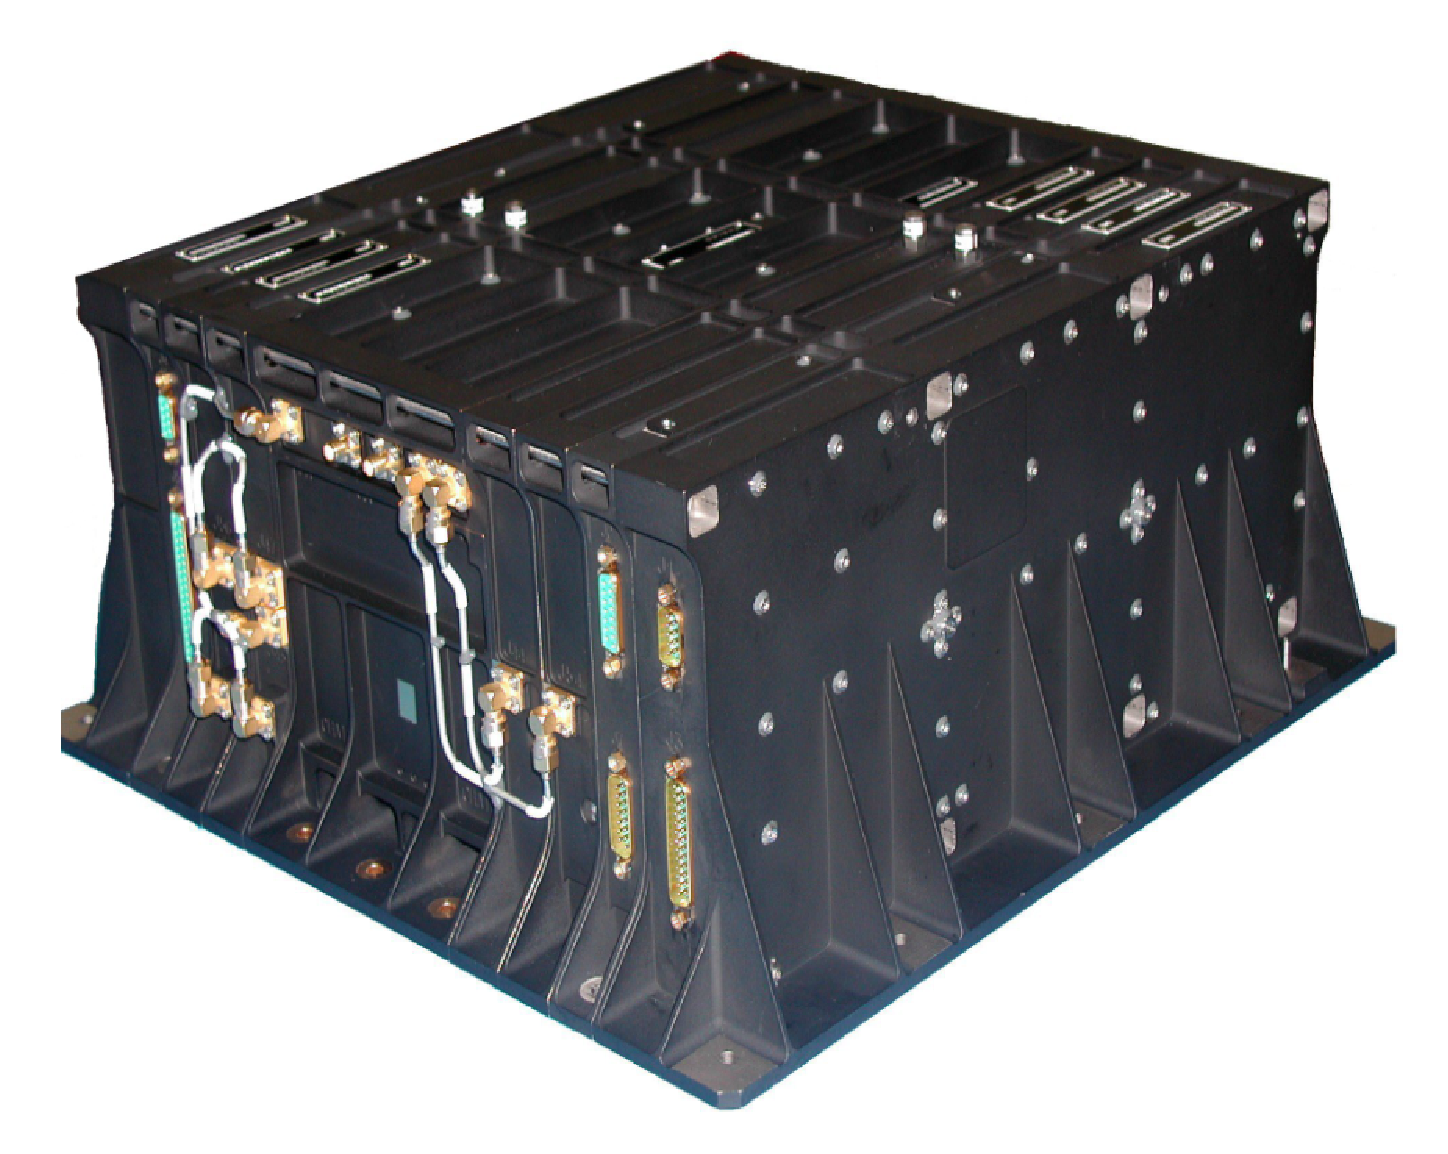
\includegraphics[width=.3\linewidth]{appendix_doris_receiver.eps}
  \caption{odbiornik}
  \label{fig:DORIS_eq_sub2}
\end{subfigure}
\begin{subfigure}{.3\textwidth}
	\centering
	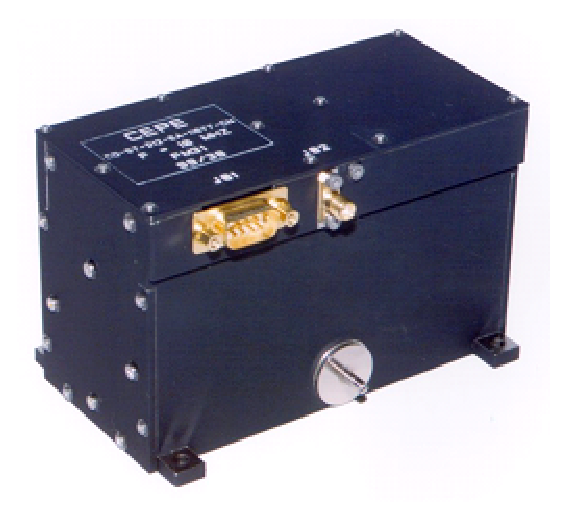
\includegraphics[width=.3\linewidth]{appendix_doris_freequency_generator.eps}
	\caption{generator częstotliwości wzorcowej}
	\label{fig:DORIS_eq_sub3}
\end{subfigure}
\caption{\textit{Komponenty systemu DORIS}
źródło: \protect\url{http://smsc.cnes.fr/DORIS/GP_systeme.htm}}
\label{fig:DORIS_equipment}
\end{figure}

\indent Kiedy satelita z zainstalowanym na pokładzie systemem DORIS zbliża się w kierunku stacji emitującej sygnal referencyjny,
częstotliwość odbieranego przez odbiornik sygnału ulega zwiększeniu. Gdy satelita oddala się od źródła sygnału wtedy odbiornik systemu DORIS 
odbiera sygnał o częstotliwości niższej niż referencyjna. Wykorzystując super stabilny wzorzec częstotliwości referencyjnej system w każdym pomiarze (interwał 10s)
porównuje częstotliwość fali elektromagnetycznej odbieranego sygnału z częstotliwością wzorca. Na podstawie pomiarów dopplerowskiej zmiany częstotliwości,
przy wykorzystaniu filatracji Kalmana oraz algorytmu całkowania numerycznego Runge-Kutta, oprogramowanie o nazwie DIODE wyznacza precyzyjnie 
pozycję oraz prędkość satelity w czasie rzeczywistym \cite[][zakładka: /DORIS system/Diode]{DORIS_AVISO}.\\
\indent Każdy z odbiorników sytemu DORIS przechowuje w pamięci wewnętrznej wszystkie wyniki pomiarów. W momęcie gdy satelita wraz z odbiornikiem 
znajdują się nad stacją referencyjną, wszystkie dane są wysyłane transmisją radiową na ziemię. Obecnie segment naziemny systemu DORIS tworzy około 
60 stacji permanentnych, nieprzerwanie emitujących sygnał referencyjny, równomiernie rozmieszczonych na powierzchni całego Globu.
Wśród stacji permanentnych, których głównym zadaniem jest umożliwianie precyzyjnego wyznaczania orbit, wyróżnić można trzy stacje główne
(Toulouse, Kourou, Harthebeesthoek),
których zadaniem jest synchronizacja czasu systemu z Międzynarodowym Czasem Atomowym (TAI). 
Poniżej na rysunku \ref{fig:doris_infrastructure} zilustrowano sieć stacji referencyjnych opisywanego systemu.
\begin{figure}[H]
\centering
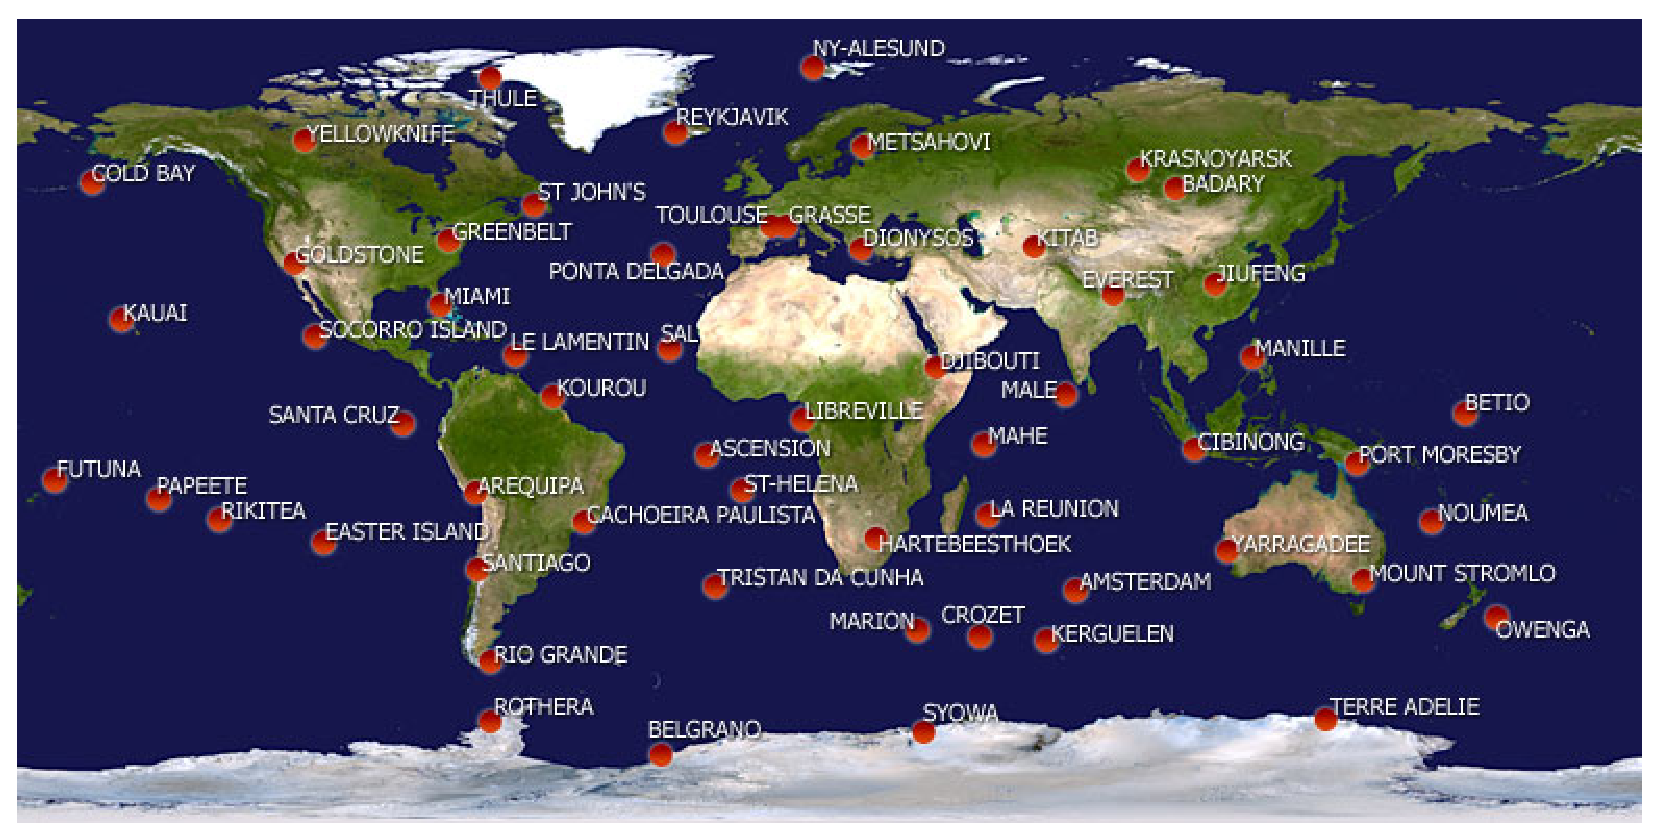
\includegraphics[scale=0.4]{appendix_doris_infrastructure.eps}
\caption{\textit{Mapa aktualnej infrastruktury naziemnej systemu DORIS} źródło: \protect\url{http://ids-doris.org/network/maps.html}}
\label{fig:doris_infrastructure}
\end{figure}
\indent Wszystkie dane zebrane przez stacje segmentu naziemnego są wysyłane do centrum obliczeniowego Ssalto
\footnote{SSALTO multi-mission altimetry, orbit determination and location ground segment (Segment-Sol multi-missions ALTimetrie, Orbitographie et localisation precise)}
w Tuluzie. W centrum obliczeniowym wyznaczane są trajektorie ruchu satelitów wyposarzonych w odbiorniki systemu DORIS. Ssalto jest również odpowiedzialne
za gromadzenie oraz dystrybucję danych pozyskanych za pomocą DORIS
\cite[][zakładka: Control and processing centre]{DORIS_AVISO}.\\
\indent Precyzyjne orbity satelitów wyznaczane za pomocą systemu DORIS znalazły szerokie zastosowanie w altimetrii geodezyjnej (badanie poziomu mórz i oceanów),
na potrzeby badania zmian klimatycznych tak bardzo istotnych dla rolnictwa. 

%%%%%%%%%%%%%%%%%%%%%%%%%%%%%%%%%%%%%%%%%%%%%%%%%%%%%%%%%%%%%%%%%%%%%%%%%%%%%%%%%%%%%%%%%%%%%%%%%
%		SLR
%%%%%%%%%%%%%%%%%%%%%%%%%%%%%%%%%%%%%%%%%%%%%%%%%%%%%%%%%%%%%%%%%%%%%%%%%%%%%%%%%%%%%%%%%%%%%%%%%
\section{SLR}
\noindent SLR (Salellite Laser Ranging)
Pomiary laserowe w których mierzy się odległości 
z stacji referencyjnej do satelitów. Wiązka laserowa odbija się od reflektorów zwrotnych umieszczonych 
na satelicie. Odległość do satelity wyznacza się mierząc czas jaki przebywa fala elektromagnetyczna o 
precyzyjnie określonej częstotliwości do satelity i z powrotem. Na podstawie pomiarów SLR wyznacza się precyzyjnie 
parametry orbit sztucznych satelitów systemów GNSS.\\
\indent Poniżej na podstawie \cite[][zakładka: Stacja Laserowa/informacje ogólne]{BOROWIEC} zaostały wypunktowane najwazniejsze zastosowania obserwacji SLR:
\begin{itemize}
\item wyznaczanie efemeryd sztucznych satelitów Ziemi z centymetrową dokładnością.
\item wyznaczanie zmiennego w czasie położenia geocentrum.
\item monitorowanie parametrów rotacji Ziemi (ruch biegunów i długość doby).
\item wyznaczanie współrzędnych oraz prędkości stacji referencyjnej wykonującej pomiar.
\item wyznaczanie parametrów Międzynarodowego Ziemskiego Układu Odniesienia ITRF oraz jego poprawę.
\end{itemize}
%%%%%%%%%%%%%%%%%%%%%%%%%%%%%%%%%%%%%%%%%%%%%%%%%%%%%%%%%%%%%%%%%%%%%%%%%%%%%%%%%%%%%%
%			LLR
%%%%%%%%%%%%%%%%%%%%%%%%%%%%%%%%%%%%%%%%%%%%%%%%%%%%%%%%%%%%%%%%%%%%%%%%%%%%%%%%%%%%%%
\section{LLR}
\noindent LLR (Lunar Laser Ranging)
Polega na pomiarze laserowym odległości do naturalnego satelity Ziemi - Księżyca.
Kosmonauci z misji Apollo15 umieścili na Księżycu reflektor zwrotny który odbija światło.  
w tym samym kierunku z którego pada źródło. Pomiar odległości wyznacza się wedle tej samej zasady jak w SLR.
Jako ciekawostkę nalezy wspomnieć, że moc lasera jest rzędu kilku gigawatów, a do Ziemi udaje się powrócić 
tylko pojedynczym fotonom.\\
\indent Pomiary te wykorzystywane są w celu wyznaczania chwilowego położenia środka cieżkości naszej planety.
Poniżej na rysunku \ref{fig:LLR_both} są przedstawione pomiary laserowe wykonywane w obserwatorium Greenbelt w USA.
\begin{figure}[H]
\centering
\begin{subfigure}{.5\textwidth}
  \centering
  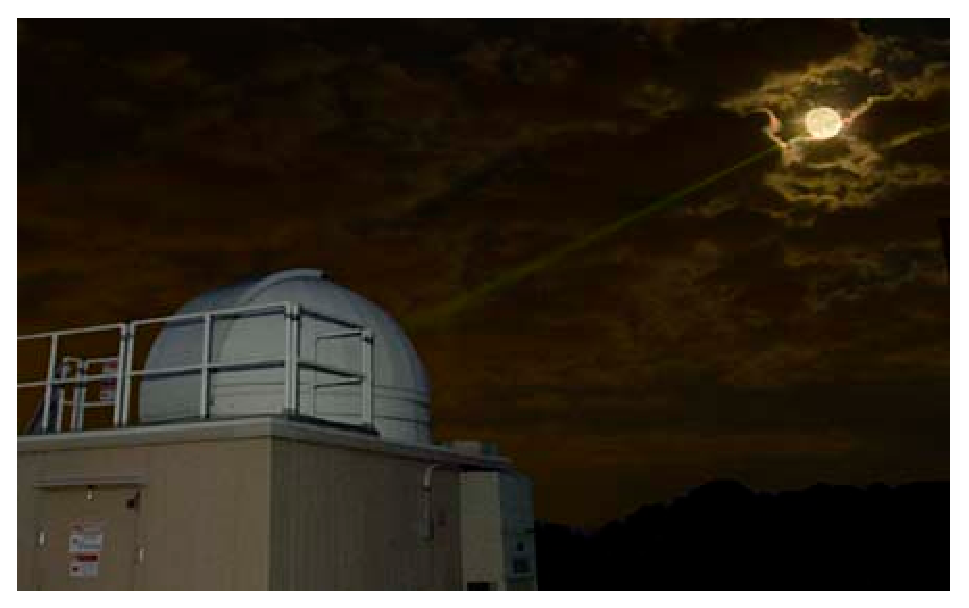
\includegraphics[width=.4\linewidth]{appendix_pomiary_laserowe.eps}
  \caption{}
  \label{fig:LLR_sub1}
\end{subfigure}%
\begin{subfigure}{.5\textwidth}
  \centering
  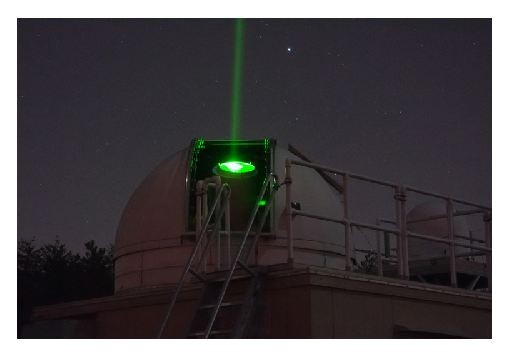
\includegraphics[width=.4\linewidth]{appendix_pomiary_laserowe2.eps}
  \caption{}
  \label{fig:LLR_sub2}
\end{subfigure}
\caption{\textit{Nocne pomiary do księzyca w obserwatorium NASA na stacji GGAO/GSFC w Greenbelt, Maryland, USA}
źródło: \protect\url{http://space-geodesy.gsfc.nasa.gov/multimedia/GeodesyNetwork/GeodesyNetworkImages.html}}
\label{fig:LLR_both}
\end{figure}
%%%%%%%%%%%%%%%%%%%%%%%%%%%%%%%%%%%%%%%%%%%%%%%%%%%%%%%%%%%%%%%%%%%%%%%%%%%%%%%%%%%%%%
% 			POLSKI WKLAD
%%%%%%%%%%%%%%%%%%%%%%%%%%%%%%%%%%%%%%%%%%%%%%%%%%%%%%%%%%%%%%%%%%%%%%%%%%%%%%%%%%%%%

\section{Polski wkład}
\noindent Warto nadmienić, że w Borowcu niedaleko Poznania znajduje się obserwatorium astrogeodynamiczne Centrum Badań Kosmicznych Polskiej Akademii Nauk, 
w którym prowadzone są globalne i lokalne badania geodynamiczne z wykorzystaniem technik GPS oraz SLR.
W ramach obserwatorium działa także grupa Służby Czasu, która partycypuje w tworzeniu międzynarodowej skali czasu atomowego TAI oraz UTC.
Utrzymanie wysokiej dokładności pomiaru czasu (błąd jest obecnie mniejszy niż 2ns) ma kluczowe znaczenie w celu zapewnienia 
wysokiej dokładności pomiarów GNSS. \cite[][zakładka: infomracje ogólne]{BOROWIEC}
\indent W ramach pomiarów SLR stacja badawcza w Borowcu prowadzi pomiary do kilkunastu sztucznych satlitów Zimi. 
W obserwarorium znajduje się także permanentna stacja IGS (jest zaangażowana w dostarczanie najwyższej jakości danych i wyników jako standardu dla Globalnego Systemu Nawigacji Satelitarnej) której odbiorniki zbierają obserwacje z satalitów GPS w sposób ciągły.
Permanentna stacja wchodzi w skład International GNSS service oraz EUREF. W ramach powyższych organizacji definiuje i realizuje Polski oraz Europejski Układ Odniesienia
\cite[][zakładka: Stacja IGS]{BOROWIEC}
 
